\documentclass[jafontsize=6bp,baselineskip=1.1zh,cmyk,landscape]{jlreq}
\usepackage{luatexja,pdfrender,xparse,fontspec,bxokumacro,bxghost}
\ltjsetparameter{jacharrange={-3,-8}}
\usepackage[no-math,match,deluxe]{luatexja-preset}
\usepackage[x-4]{pdfx}
\usepackage[margin=10mm]{geometry}
\usepackage{tikz}
\usetikzlibrary{calc,fadings,patterns,arrows.meta}
\setlength{\parskip}{0pt}

\NewDocumentCommand\hmfukuro{O{.2pt} +m O{white}}{\textpdfrender{
	TextRenderingMode=FillStroke,
	LineWidth=#1,
	FillColor=#3,
}{#2}}

\newlength{\OrigWidth}
%% \hminwidth[*]{«横幅»}{«テキスト»}
% テキストを指定の横幅に"イイカンジに"出力する
% *-> 均等割り付けしない
\NewDocumentCommand\hminwidth{s m m}{{%
	\settowidth{\OrigWidth}{#3}% \settowidth 便利
	\ifthenelse{\lengthtest{\OrigWidth > #2}}{%
		% 指定幅より大きい場合は横方向に縮小する
		\resizebox{#2}{\height}{#3}% 横幅だけ変える
	}{%else
		\IfBooleanTF{#1}{%
			% * 付きで指定幅以下ならそのまま出力
			#3
		}{%
			% 指定幅以下の場合は均等割りを行う
			\kintou{#2}{\jghostguarded{}#3\jghostguarded{}}%
		}%
	}%
}}

\setmainfont{FOT-MatissePro-M}\setmainjfont{FOT-MatissePro-M}
\setsansfont{FOT-RodinNTLGPro-DB}\setsansjfont{FOT-RodinNTLGPro-DB}
\newfontfamily\hmcfont[Scale=0.9]{NKD04_Playing_Cards_Index}
\newfontfamily\hmtfont[Scale=1.2]{kawoszeh}
\newfontfamily\hmgfont[Scale=0.9]{NKD04_Playing_Cards_Index}
\newfontfamily\hmgcfont[Scale=1.2]{kawoszeh}
\newjfontfamily\hmsjfont[Scale=1.0]{FOT-RodinNTLGPro-UB}
\newfontfamily\hmsafont[Scale=1.0]{FOT-RodinNTLGPro-UB}
\newcommand{\hmsfont}{\hmsafont\hmsjfont}
\newfontfamily\hmpfont[Scale=1.2]{Hall Fetica Upper}
\newfontfamily\hmnafont{FOT-TsukuOldGothicStd-B}
\newjfontfamily\hmnjfont{FOT-TsukuOldGothicStd-B}
\newcommand{\hmnfont}{\hmnafont\hmnjfont}
% \newfontfamily\hmxafont{FOT-TsukuOldGothicStd-B}
% \newjfontfamily\hmxjfont{FOT-TsukuOldGothicStd-B}
% \newcommand{\hmxfont}{\hmxafont\hmxjfont}
\newfontfamily\nishikiafont{nishiki-teki}
\newjfontfamily\nishikijfont{nishiki-teki}
\newcommand{\nishikifont}{\nishikiafont\nishikijfont}

\colorlet{nodecolor}{violet!90!blue}
\colorlet{costcolor}{olive!30!black}
\colorlet{spiritcolor}{red!70!black}
\colorlet{grazecolor}{yellow!70!black}
\colorlet{rangebcolor}{black!90}
\colorlet{rangecolor}{black!10}
\colorlet{characolor}{teal!60}
\colorlet{spellcolor}{orange!60}
\colorlet{commandcolor}{gray!60}
\colorlet{gridcolor}{cyan!60}

\colorlet{icoAcolor}{violet}
\colorlet{icoBcolor}{orange}
\colorlet{icoCcolor}{magenta}
\colorlet{icoDcolor}{olive}
\colorlet{icoEcolor}{green}
\colorlet{icoFcolor}{lime}
\colorlet{icoGcolor}{red}
\colorlet{icoHcolor}{teal}
\colorlet{icoIcolor}{cyan}
\colorlet{icoLcolor}{yellow}
\colorlet{icoJcolor}{gray}
\colorlet{icoLcolor}{darkgray}

\newcommand{\hmicoA}{{\color{icoAcolor}\jfontspec{nishiki-teki}\fontspec{nishiki-teki}\char"0262F}}
\newcommand{\hmicoB}{{\color{icoBcolor}\jfontspec{nishiki-teki}\fontspec{nishiki-teki}\char"1F3DA}}
\newcommand{\hmicoC}{{\color{icoCcolor}\jfontspec{nishiki-teki}\fontspec{nishiki-teki}\char"1F571}}
\newcommand{\hmicoD}{{\color{icoDcolor}\jfontspec{nishiki-teki}\fontspec{nishiki-teki}\char"026F0}}
\newcommand{\hmicoE}{{\color{icoEcolor}\jfontspec{nishiki-teki}\fontspec{nishiki-teki}\char"1F407}}
\newcommand{\hmicoF}{{\color{icoFcolor}\jfontspec{nishiki-teki}\fontspec{nishiki-teki}\char"1F3A9}}
\newcommand{\hmicoG}{{\color{icoGcolor}\jfontspec{nishiki-teki}\fontspec{nishiki-teki}\char"1F3F0}}
\newcommand{\hmicoH}{{\color{icoHcolor}\jfontspec{nishiki-teki}\fontspec{nishiki-teki}\char"1F408}}
\newcommand{\hmicoI}{{\color{icoIcolor}\jfontspec{nishiki-teki}\fontspec{nishiki-teki}\char"1F326}}
\newcommand{\hmicoJ}{{\color{icoLcolor}\jfontspec{nishiki-teki}\fontspec{nishiki-teki}\char"1F318}}
\newcommand{\hmicoK}{{\color{icoJcolor}\jfontspec{nishiki-teki}\fontspec{nishiki-teki}\char"1F47B}}
\newcommand{\hmicoL}{{\color{icoLcolor}\jfontspec{nishiki-teki}\fontspec{nishiki-teki}\char"1F3E2}}
\newcommand{\hmicot}{{\jfontspec{nishiki-teki}\fontspec{nishiki-teki}\char"1F5E1}}
\newcommand{\hmicoo}{{\jfontspec{nishiki-teki}\fontspec{nishiki-teki}\char"1F300}}
\newcommand{\hmicoa}{{\jfontspec{nishiki-teki}\fontspec{nishiki-teki}\char"0272C}}
\newcommand{\hmicov}{{\jfontspec{nishiki-teki}\fontspec{nishiki-teki}\char"0292D}}
\newcommand{\hmicoi}{{\jfontspec{nishiki-teki}\fontspec{nishiki-teki}\char"026C8}}
\newcommand{\hmicom}{{\jfontspec{nishiki-teki}\fontspec{nishiki-teki}\char"1F570}}
\newcommand{\hmicoc}{{\jfontspec{nishiki-teki}\fontspec{nishiki-teki}\char"1F3AD}}
\newcommand{\hmicoe}{{\jfontspec{nishiki-teki}\fontspec{nishiki-teki}\char"02694}}
\newcommand{\hmicow}{{\jfontspec{nishiki-teki}\fontspec{nishiki-teki}\char"1F342}}
\newcommand{\hmicos}{{\jfontspec{nishiki-teki}\fontspec{nishiki-teki}\char"1F54B}}
\newcommand{\hmicox}{{\jfontspec{nishiki-teki}\fontspec{nishiki-teki}\char"0254D}}

\newcommand{\©}{\jghostguarded{©}}
\newcommand{\・}{\mbox{・}}
\newcommand{\↓}{{\fontspec{nishiki-teki}⤸}}



\setlength{\parindent}{0pt}

\begin{document}
%: キャラ
\begin{tikzpicture}[x=1mm,y=1mm]
	% 座標
	\coordinate(OL1)at(63,88);\coordinate(OL3)at(0,0);
	\coordinate(N1)at(10,86);\coordinate(N3)at(2,78);
	\coordinate(N2)at(N1-|N3);\coordinate(N4)at(N1|-N3);
	\coordinate(C1)at(16,82);\coordinate(C3)at(8,74);
	\coordinate(C2)at(C1-|C3);\coordinate(C4)at(C1|-C3);
	\coordinate(TC)at(12,84);
	\coordinate(SC)at(49,82);\coordinate(GC)at(56,81);
	\coordinate(SC2)at(51,82);\coordinate(GC2)at(57,82);
	\coordinate(B1)at(59,30);\coordinate(B3)at(4,6);
	\coordinate(B3*)at($(B3)+(0,4)$);
	\coordinate(I1)at(59,84);\coordinate(I3)at(10,32);
	\coordinate(O1)at(61,86);\coordinate(O3)at(2,2);
	\coordinate(MT)at(5,78);\coordinate(M1)at(10,78);\coordinate(M3)at(2,30);
	\coordinate(RT)at(9,74);
	% 枠
	% 外枠
	\draw(O1)rectangle(O3);
	\fill[black](OL1)-|(OL3)-|cycle (O1)|-(O3)|-cycle;
	\fill[spellcolor](O1)-|(O3)-|cycle;
	\draw[path picture={\node at (path picture bounding box.center)
		{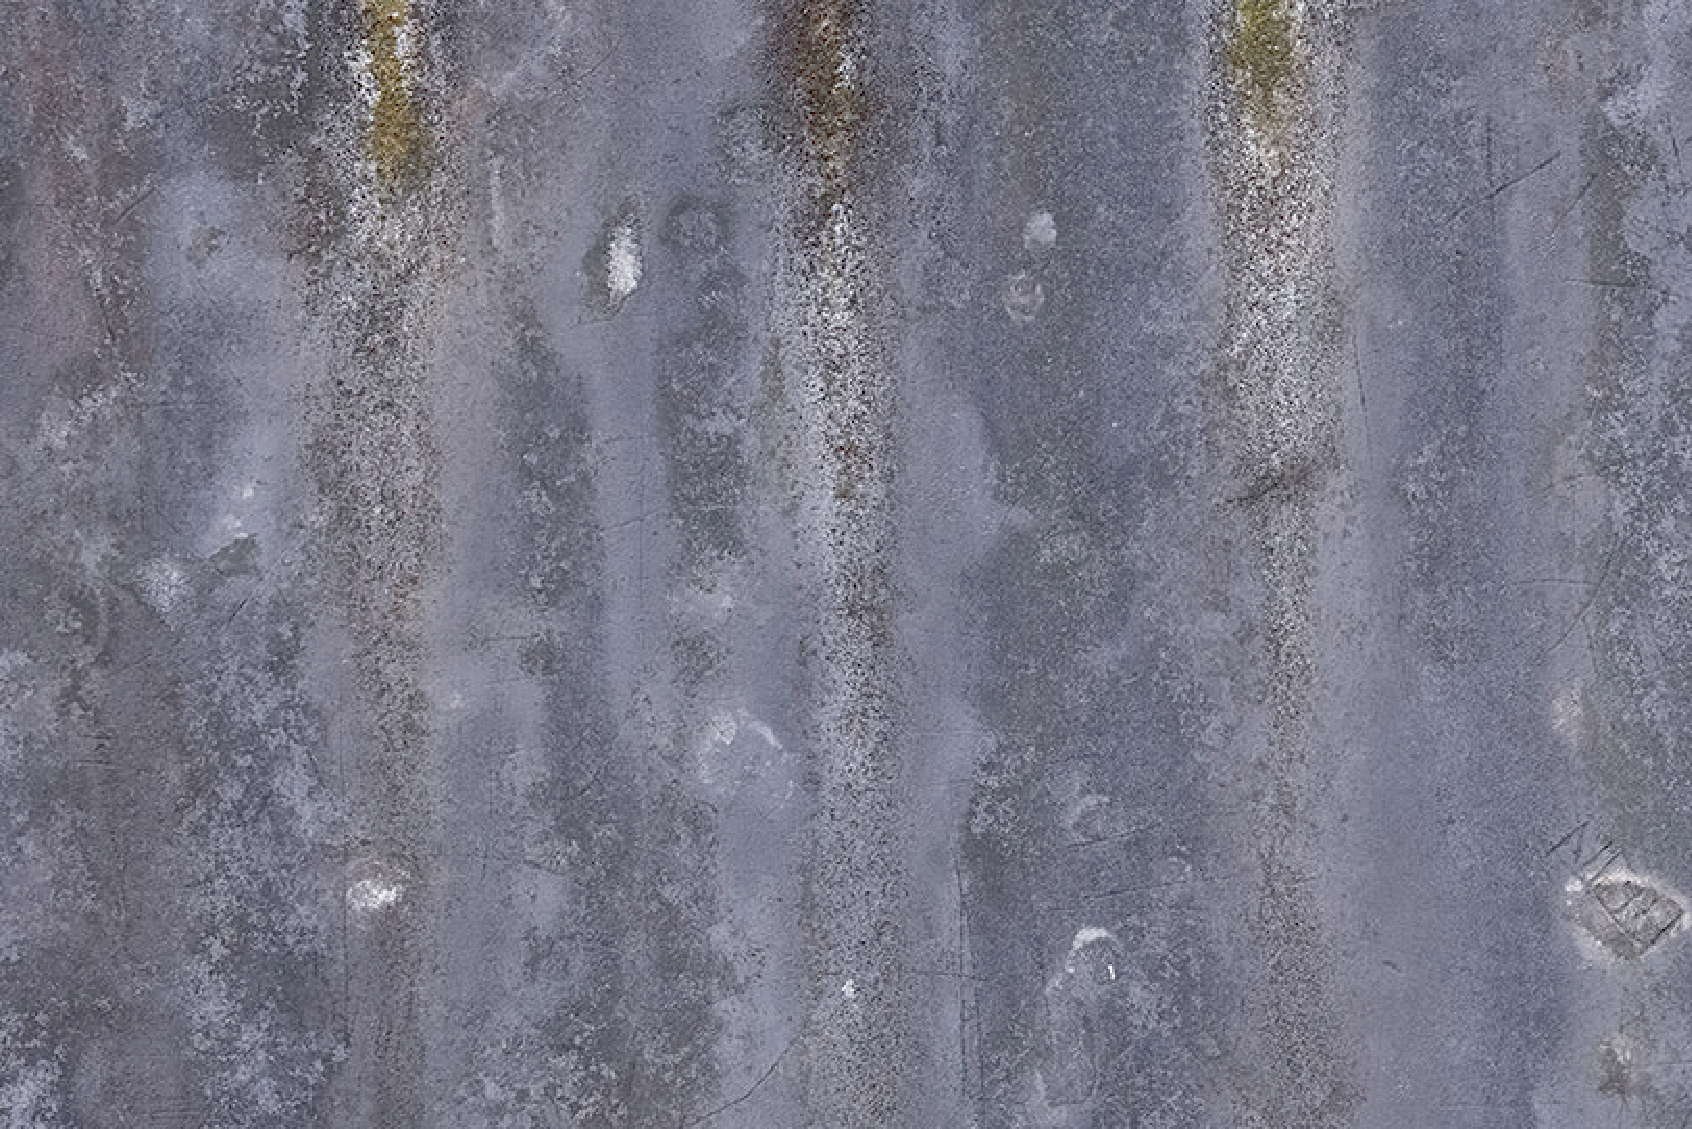
\includegraphics[height=88mm]{ch_back.pdf}};}](O1)-|(O3)-|cycle;
	% イラスト
	\draw[path picture={\node at (path picture bounding box.center)
		{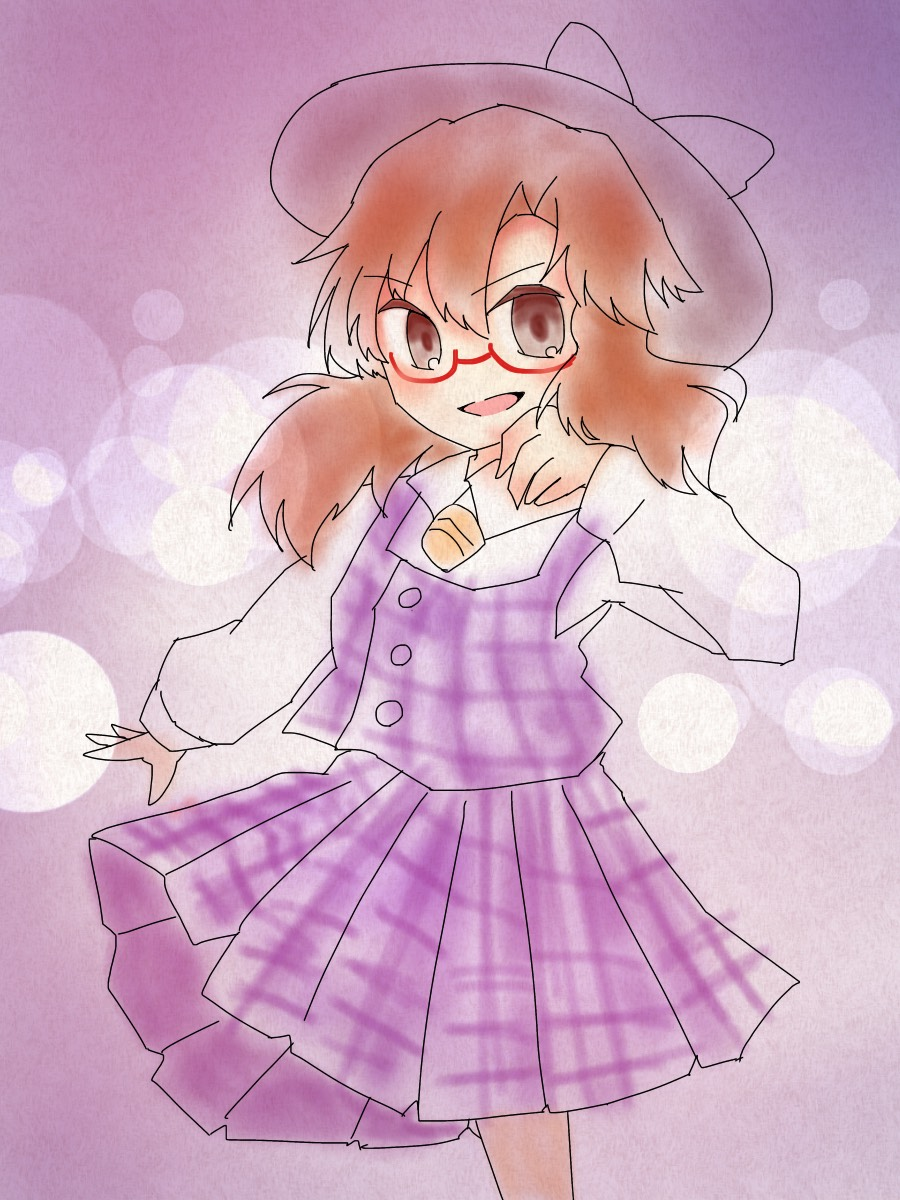
\includegraphics[width=49mm]{sumire.jpg}};}](I1)rectangle(I3);
	%\draw[path picture={\node at (path picture bounding box.center)
		%{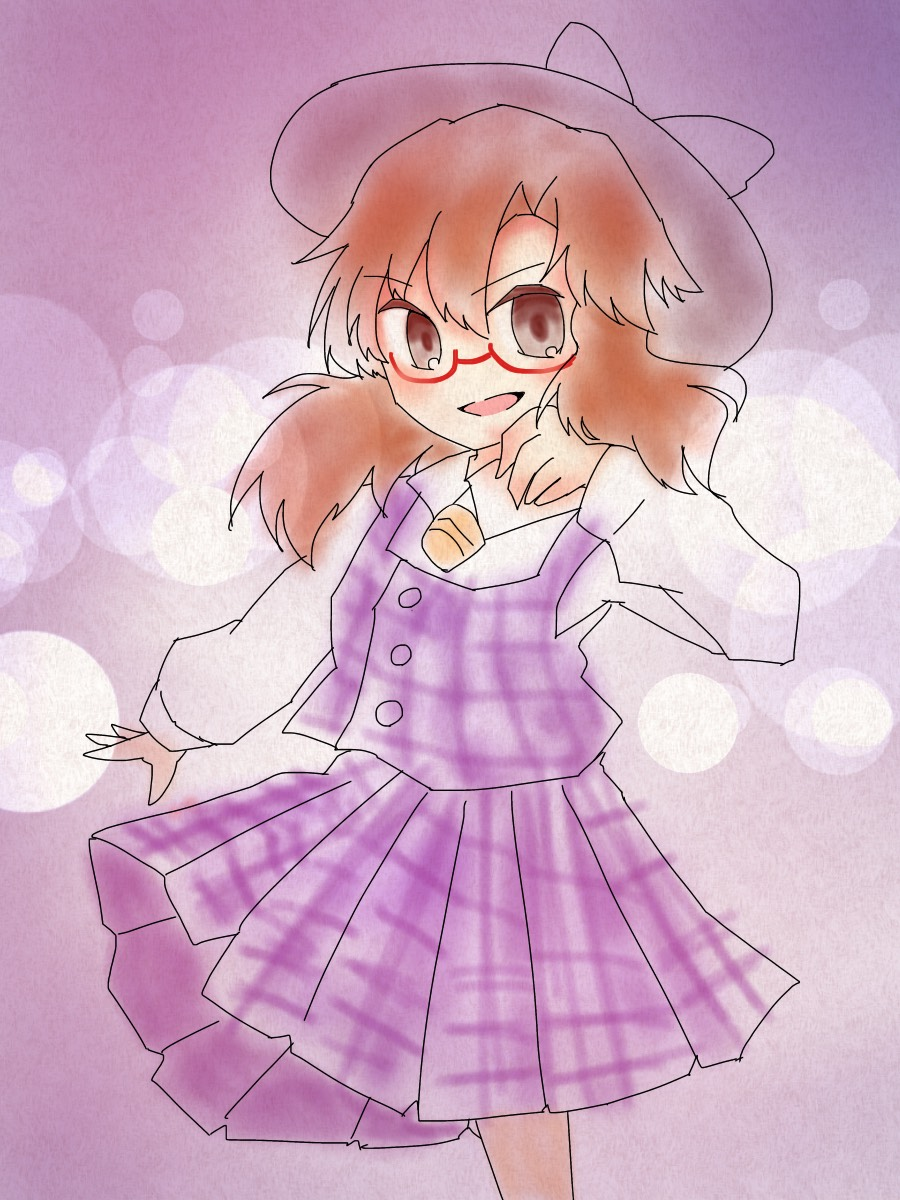
\includegraphics[height=88mm]{sumire.jpg}};}](OL1)rectangle(OL3);
	% カード名
	\fill[black,path fading=west](M1)rectangle(M3);
	\path(MT)node[below,inner sep=0,outer sep=0]
		{\hbox{\tate\hminwidth{48mm}{\fontsize{6mm}{0}\hmnfont\hmfukuro[.3pt]{宇佐見 菫子}}}};
	\path(RT)node[below,white,inner sep=0,outer sep=0]
		{\hbox{\tate\hminwidth*{44mm}{\fontsize{2mm}{0}\hmnfont うさみ すみれこ}}};
	% タイプ、術者
	\filldraw[fill=characolor!50,draw=characolor](TC)circle[radius=1.9];
	\draw(TC)node{\hmtfont{Ch}};
	\path(TC)--++(2,0)node[right]{\hmsfont\hmfukuro{}};
	% コスト
	\filldraw[fill=costcolor!30,draw=costcolor,thick](C1)rectangle(C3);
	\fill[fill=costcolor!70]
		($(C1)!.5!(C2)$)--($(C2)!.5!(C3)$)--($(C3)!.5!(C4)$)--($(C4)!.5!(C1)$)--cycle
		(C1)-|(C3)|-cycle;
	\path(C1)|-(C3)node[near end,above,outer ysep=0]{\hmcfont\small COST};
	\path(C1)--(C3)node[midway]{\hmcfont\Huge\hmfukuro{2}};
	% ノード
	\filldraw[fill=nodecolor!30,draw=nodecolor,thick](N1)rectangle(N3);
	\fill[fill=nodecolor!70](N1)--(N3)--(N4)--(N2)--cycle;
	\path(N1)-|(N3)node[near start,below,outer ysep=0]{\hmcfont\small NODE};
	\path(N1)--(N3)node[midway]{\hmcfont\Huge\hmfukuro{5}};
	% 霊力
	\filldraw[fill=spiritcolor!40,draw=spiritcolor,thick](SC)circle[radius=3];
	\fill[fill=spiritcolor!10](SC)circle[radius=2];
	\path(SC)--++(0,2.5)node{\small\hmgcfont\hmfukuro{\strut Spirit}};
	\path(SC)node{\LARGE\hmgfont 3};
	% グレイズ
	\fill[fill=grazecolor!10](GC)circle[radius=4.5];
	\fill[fill=grazecolor!40](GC)--++(-45:4.5)arc(315:135:4.5)--cycle;
	\draw[draw=grazecolor,thick](GC)circle[radius=4.5];
	\path(GC)--++(0,3.5)node{\small\hmgcfont\hmfukuro{\strut Graze}};
	\path(GC)node{\Huge\hmgfont 3};
	% % 発動期間
	% \filldraw[fill=rangebcolor,draw=rangebcolor!80,thick](SC2)circle[radius=2.5];
	% \path(SC2)node[rangecolor]{\LARGE\hmicot};
	% % 効果範囲
	% \filldraw[fill=rangebcolor,draw=rangebcolor!80,thick](GC2)circle[radius=2.5];
	% \path(GC2)node[rangecolor]{\LARGE\hmicom};
	% 種族
	\path(I3)-|(I1)node[midway,above left]{\large\hmsfont\hmfukuro{人間}};
	% テキスト
	\draw[fill=icoLcolor!30,fill opacity=.85](B1)rectangle(B3);
	%% 場所
	\path(B1)--(B3)node[midway,text opacity=.3]{\fontsize{20mm}{0}\hmicoL};
	%% テキスト
	\path(B1)-|(B3)node[
		midway,below right,outer sep=0,inner sep=1mm,text width=53mm,text justified,font=\small\sffamily]{
			(自動γ)〔このキャラクター〕にセットされているカードが 7 枚以上になった場合、
			〔このキャラクターにセットされているカード全て〕を破棄する。その後、この効果で
			破棄したカードから 1 枚選んで、あなたがプレイしたものとして解決する。
			
			(自分ターン)[2]\↓: 目標の〔あなたの冥界にあるカード 1 枚〕を〔このキャラクター〕
			にセットする。
		};
	%% 戦闘力
	\path($(B1)-(7,0)$)|-(B3)node
		[midway,above,outer sep=0,inner xsep=0,inner ysep=1mm,text width=14mm,text centered,font=\LARGE\hmpfont]
		{\mbox{\makebox[4mm][r]{3}/\makebox[4mm][l]{5}}};
	%% フレーバーテキスト
	\path(B3)node[above right,outer sep=0,inner sep=1mm,text width=39mm,text justified,font=\scriptsize]{
			「どういうこと? これからどうなるの?」
		};
	% フッター
	\path(O3)node[above right,text width=10\zw,align=left,inner ysep=0,outer ysep=0]
		{\hmfukuro{\scriptsize\hmsfont{\©}上海アリス幻樂団\\[-3pt]{\©}さーくる⑨}};
	\path(O1)|-(O3)node[pos=.75,above left,inner xsep=0,outer xsep=0]{\hmpfont\small\hmfukuro{No.~}};
	\path(O1)|-(O3)node[pos=.75,above right,inner xsep=0,outer xsep=0]{\hmpfont\small\hmfukuro{0001}};
	\path(O1)|-(O3)node[pos=.68,above]{\hmpfont\small\hmfukuro{<S>}};
	\path(O1)|-(O3)node[midway,above left]{\hmsfont\small\hmfukuro{Ill. 湯島}};
	% % 方眼
	% \draw[very thin,gridcolor,nearly transparent](OL1)grid[step=1](OL3);
	% \draw[gridcolor,nearly transparent]($(OL1)-(2,2)$)rectangle($(OL3)+(2,2)$);
	% \draw[thin,gridcolor,nearly transparent](OL1)grid[step=10](OL3);
	% \draw[thin,gridcolor,nearly transparent](OL1)rectangle(OL3);
\end{tikzpicture}
\hfill
%: スペル
\begin{tikzpicture}[x=1mm,y=1mm]
	% 座標
	\coordinate(OL1)at(63,88);\coordinate(OL3)at(0,0);
	\coordinate(N1)at(10,86);\coordinate(N3)at(2,78);
	\coordinate(N2)at(N1-|N3);\coordinate(N4)at(N1|-N3);
	\coordinate(C1)at(16,82);\coordinate(C3)at(8,74);
	\coordinate(C2)at(C1-|C3);\coordinate(C4)at(C1|-C3);
	\coordinate(TC)at(12,84);
	\coordinate(SC)at(49,82);\coordinate(GC)at(56,81);
	\coordinate(B1)at(59,30);\coordinate(B3)at(4,6);
	\coordinate(B3*)at($(B3)+(0,4)$);
	\coordinate(I1)at(59,84);\coordinate(I3)at(10,32);
	\coordinate(O1)at(61,86);\coordinate(O3)at(2,2);
	\coordinate(MT)at(5,78);\coordinate(M1)at(10,78);\coordinate(M3)at(2,30);
	\coordinate(RT)at(9,74);
	% 枠
	% 外枠
	\draw(O1)rectangle(O3);
	\fill[black](OL1)-|(OL3)-|cycle (O1)|-(O3)|-cycle;
	\fill[spellcolor](O1)-|(O3)-|cycle;
	\draw[path picture={\node at (path picture bounding box.center)
		{\includegraphics[height=88mm]{sc_back.pdf}};}](O1)-|(O3)-|cycle;
	% イラスト
	\draw[path picture={\node at (path picture bounding box.center)
		{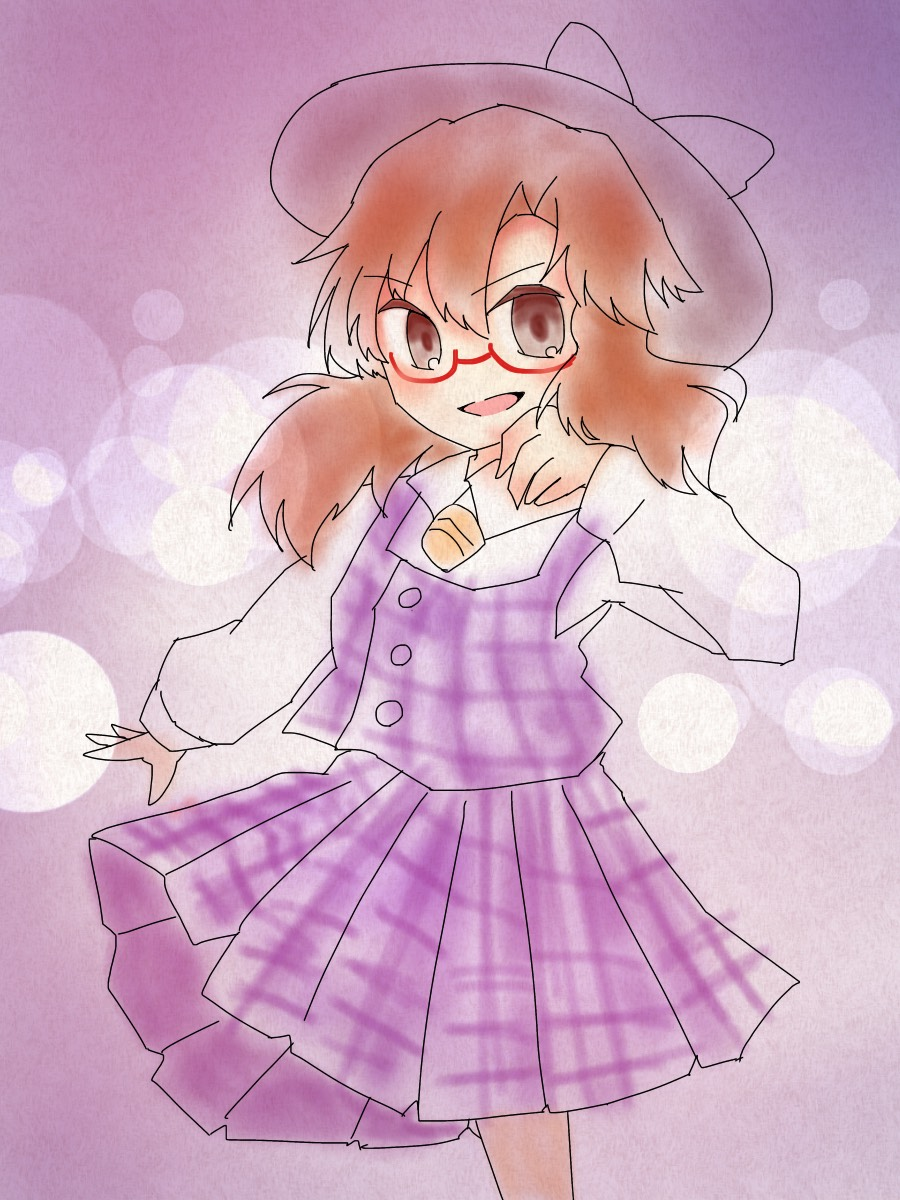
\includegraphics[width=49mm]{sumire.jpg}};}](I1)rectangle(I3);
	%\draw[path picture={\node at (path picture bounding box.center)
		%{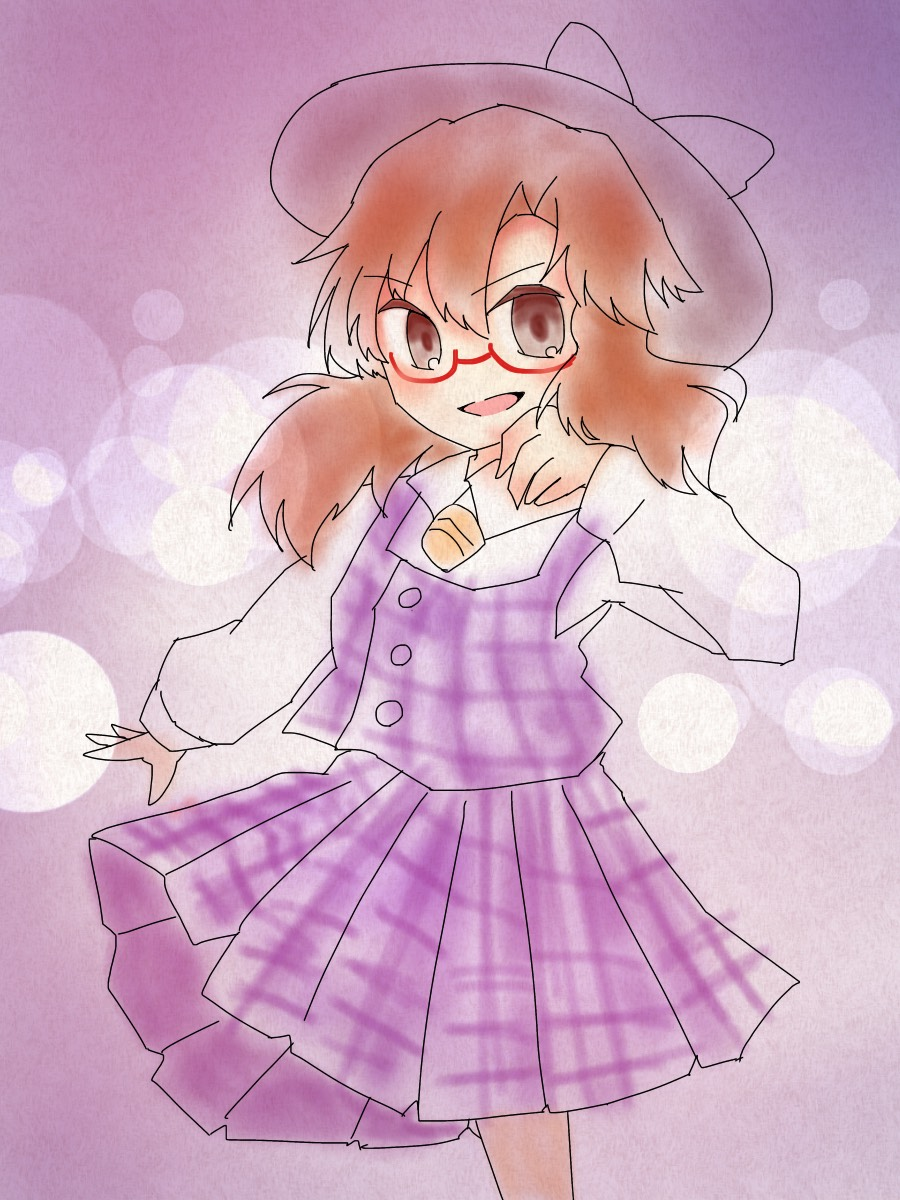
\includegraphics[height=88mm]{sumire.jpg}};}](OL1)rectangle(OL3);
	% カード名
	\fill[black,path fading=west](M1)rectangle(M3);
	\path(MT)node[below,inner sep=0,outer sep=0]
		{\hbox{\tate\hminwidth{48mm}{\fontsize{6mm}{0}\hmnfont\hmfukuro[.3pt]{念力「テレキネシス 電波塔」}}}};
	\path(RT)node[below,white,inner sep=0,outer sep=0]
		{\hbox{\tate\hminwidth*{44mm}{\fontsize{2mm}{0}\hmnfont てれきねしす でんぱとう}}};
	% タイプ、術者
	\filldraw[fill=spellcolor!50,draw=spellcolor](TC)circle[radius=1.9];
	\draw(TC)node{\hmtfont{SC}};
	\path(TC)--++(2,0)node[right]{\hmsfont\hmfukuro{宇佐見菫子}};
	% コスト
	\filldraw[fill=costcolor!30,draw=costcolor,thick](C1)rectangle(C3);
	\fill[fill=costcolor!70]
		($(C1)!.5!(C2)$)--($(C2)!.5!(C3)$)--($(C3)!.5!(C4)$)--($(C4)!.5!(C1)$)--cycle
		(C1)-|(C3)|-cycle;
	\path(C1)|-(C3)node[near end,above,outer ysep=0]{\hmcfont\small COST};
	\path(C1)--(C3)node[midway]{\hmcfont\Huge\hmfukuro{2}};
	% ノード
	\filldraw[fill=nodecolor!30,draw=nodecolor,thick](N1)rectangle(N3);
	\fill[fill=nodecolor!70](N1)--(N3)--(N4)--(N2)--cycle;
	\path(N1)-|(N3)node[near start,below,outer ysep=0]{\hmcfont\small NODE};
	\path(N1)--(N3)node[midway]{\hmcfont\Huge\hmfukuro{5}};
	% % 霊力
	% \filldraw[fill=spiritcolor!40,draw=spiritcolor,thick](SC)circle[radius=3];
	% \fill[fill=spiritcolor!10](SC)circle[radius=2];
	% \path(SC)--++(0,2.5)node{\small\hmgcfont\hmfukuro{\strut Spirit}};
	% \path(SC)node{\LARGE\hmgfont I};
	% % グレイズ
	% \fill[fill=grazecolor!10](GC)circle[radius=4.5];
	% \fill[fill=grazecolor!40](GC)--++(-45:4.5)arc(315:135:4.5)--cycle;
	% \draw[draw=grazecolor,thick](GC)circle[radius=4.5];
	% \path(GC)--++(0,3.5)node{\small\hmgcfont\hmfukuro{\strut Graze}};
	% \path(GC)node{\Huge\hmgfont +};
	% 発動期間
	\filldraw[fill=rangebcolor,draw=rangebcolor!80,thick](SC2)circle[radius=2.5];
	\path(SC2)node[rangecolor]{\LARGE\hmicom};
	% 効果範囲
	\filldraw[fill=rangebcolor,draw=rangebcolor!80,thick](GC2)circle[radius=2.5];
	\path(GC2)node[rangecolor]{\LARGE\hmicot};
	% 種族
	\path(I3)-|(I1)node[midway,above left]{\large\hmsfont\hmfukuro{}};
	% テキスト
	\draw[fill=icoHcolor!30,fill opacity=.85](B1)rectangle(B3);
	%% 場所
	\path(B1)--(B3)node[midway,text opacity=.3]{\fontsize{20mm}{0}\hmicoH};
	%% テキスト
	\path(B1)-|(B3)node[
		midway,below right,outer sep=0,inner sep=1mm,text width=53mm,text justified,font=\small\sffamily]{
			(プレイ)目標の〔キャラクター 1 枚〕に 3 ダメージを与え、スリープ状態にする。
			このフェイズ終了時に、そのキャラクターにさらに 3 ダメージを与える。
		};
	%% 戦闘力
	\path($(B1)-(7,0)$)|-(B3)node
		[midway,above,outer sep=0,inner xsep=0,inner ysep=1mm,text width=14mm,text centered,font=\LARGE\hmpfont]
		{\mbox{\makebox[4mm][r]{-}/\makebox[4mm][l]{-}}};
	%% フレーバーテキスト
	\path(B3)node[above right,outer sep=0,inner sep=1mm,text width=39mm,text justified,font=\scriptsize]{
			電波塔は電波を送信する塔のことであり、電波干渉や建造物による電波遮蔽を
			避けるため、周囲の建物よりも高く建てられる。
		};
	% フッター
	\path(O3)node[above right,text width=10\zw,align=left,inner ysep=0,outer ysep=0]
		{\hmfukuro{\scriptsize\hmsfont{\©}上海アリス幻樂団\\[-3pt]{\©}さーくる⑨}};
	\path(O1)|-(O3)node[pos=.75,above left,inner xsep=0,outer xsep=0]{\hmpfont\small\hmfukuro{No.~}};
	\path(O1)|-(O3)node[pos=.75,above right,inner xsep=0,outer xsep=0]{\hmpfont\small\hmfukuro{1111}};
	\path(O1)|-(O3)node[pos=.68,above]{\hmpfont\small\hmfukuro{<S>}};
	\path(O1)|-(O3)node[midway,above left]{\hmsfont\small\hmfukuro{Ill. 湯島}};
	% % 方眼
	% \draw[very thin,gridcolor,nearly transparent](OL1)grid[step=1](OL3);
	% \draw[gridcolor,nearly transparent]($(OL1)-(2,2)$)rectangle($(OL3)+(2,2)$);
	% \draw[thin,gridcolor,nearly transparent](OL1)grid[step=10](OL3);
	% \draw[thin,gridcolor,nearly transparent](OL1)rectangle(OL3);
\end{tikzpicture}
\hfill
%: コマンド
\begin{tikzpicture}[x=1mm,y=1mm]
	% 座標
	\coordinate(OL1)at(63,88);\coordinate(OL3)at(0,0);
	\coordinate(N1)at(10,86);\coordinate(N3)at(2,78);
	\coordinate(N2)at(N1-|N3);\coordinate(N4)at(N1|-N3);
	\coordinate(C1)at(16,82);\coordinate(C3)at(8,74);
	\coordinate(C2)at(C1-|C3);\coordinate(C4)at(C1|-C3);
	\coordinate(TC)at(12,84);
	\coordinate(SC)at(49,82);\coordinate(GC)at(56,81);
	\coordinate(B1)at(59,30);\coordinate(B3)at(4,6);
	\coordinate(B3*)at($(B3)+(0,4)$);
	\coordinate(I1)at(59,84);\coordinate(I3)at(10,32);
	\coordinate(O1)at(61,86);\coordinate(O3)at(2,2);
	\coordinate(MT)at(5,78);\coordinate(M1)at(10,78);\coordinate(M3)at(2,30);
	\coordinate(RT)at(9,74);
	% 枠
	% 外枠
	\draw(O1)rectangle(O3);
	\fill[black](OL1)-|(OL3)-|cycle (O1)|-(O3)|-cycle;
	\fill[spellcolor](O1)-|(O3)-|cycle;
	\draw[path picture={\node at (path picture bounding box.center)
		{\includegraphics[height=88mm]{cm_back.pdf}};}](O1)-|(O3)-|cycle;
	% イラスト
	\draw[path picture={\node at (path picture bounding box.center)
		{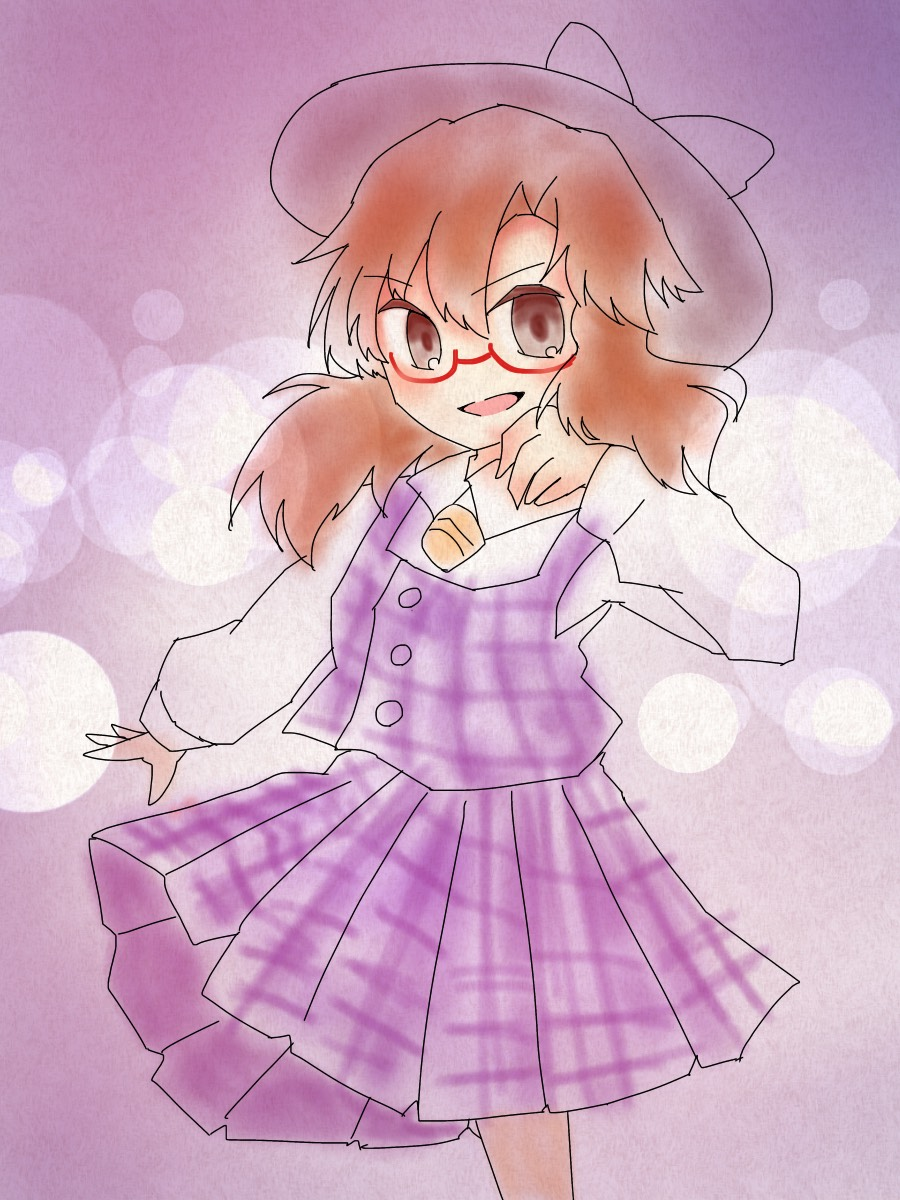
\includegraphics[width=49mm]{sumire.jpg}};}](I1)rectangle(I3);
	%\draw[path picture={\node at (path picture bounding box.center)
		%{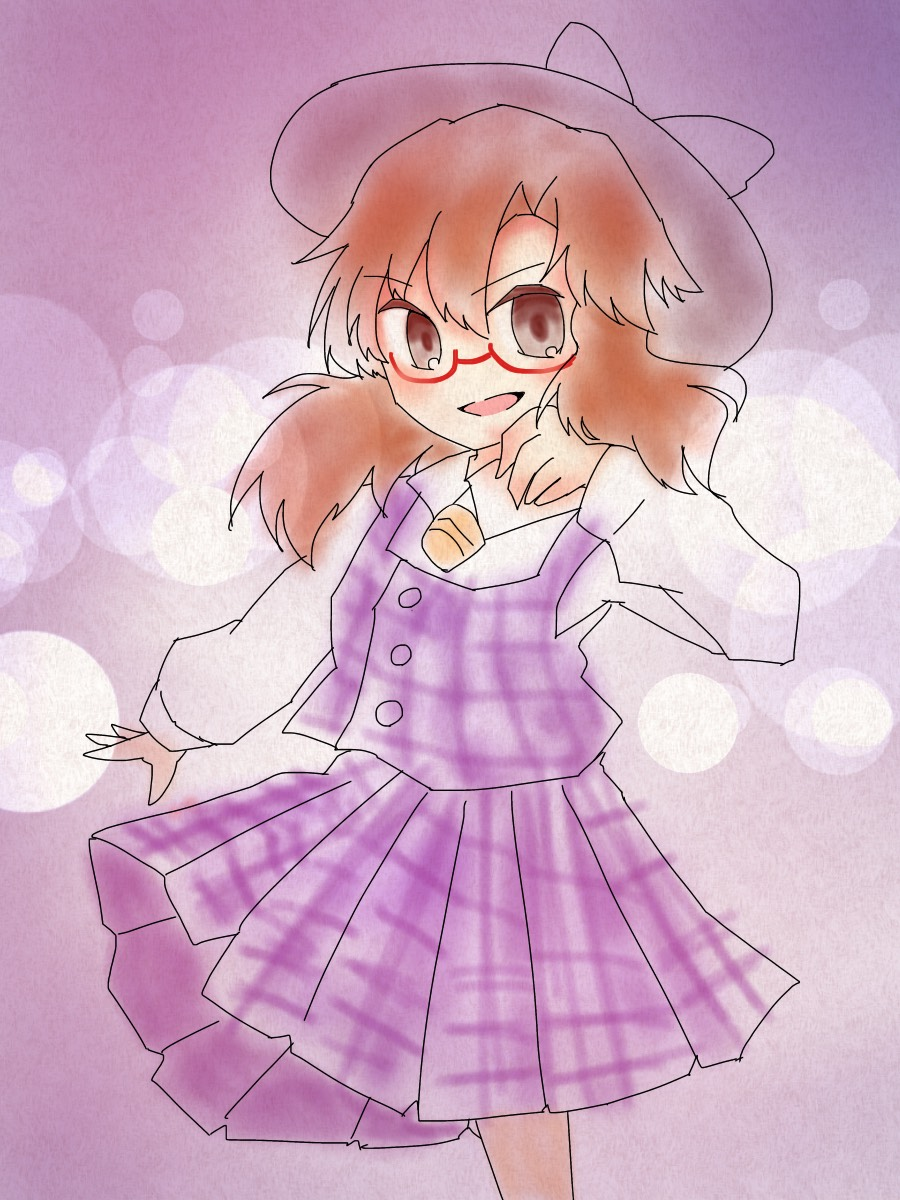
\includegraphics[height=88mm]{sumire.jpg}};}](OL1)rectangle(OL3);
	% カード名
	\fill[black,path fading=west](M1)rectangle(M3);
	\path(MT)node[below,inner sep=0,outer sep=0]
		{\hbox{\tate\hminwidth{48mm}{\fontsize{6mm}{0}\hmnfont\hmfukuro[.3pt]{ルーン文字}}}};
	\path(RT)node[below,white,inner sep=0,outer sep=0]
		{\hbox{\tate\hminwidth*{44mm}{\fontsize{2mm}{0}\hmnfont るーんもじ}}};
	% タイプ、術者
	\filldraw[fill=commandcolor!50,draw=commandcolor](TC)circle[radius=1.9];
	\draw(TC)node{\hmtfont{Cm}};
	\path(TC)--++(2,0)node[right]{\hmsfont\hmfukuro{}};
	% コスト
	\fill[fill=costcolor!30,draw=costcolor,thick](C1)rectangle(C3);
	\fill[fill=costcolor!70]
		($(C1)!.5!(C2)$)--($(C2)!.5!(C3)$)--($(C3)!.5!(C4)$)--($(C4)!.5!(C1)$)--cycle
		(C1)-|(C3)|-cycle;
	\path(C1)|-(C3)node[near end,above,outer ysep=0]{\hmcfont\small COST};
	\path(C1)--(C3)node[midway]{\hmcfont\Huge\hmfukuro{0}};
	% ノード
	\filldraw[fill=nodecolor!30,draw=nodecolor,thick](N1)rectangle(N3);
	\fill[fill=nodecolor!70](N1)--(N3)--(N4)--(N2)--cycle;
	\path(N1)-|(N3)node[near start,below,outer ysep=0]{\hmcfont\small NODE};
	\path(N1)--(N3)node[midway]{\hmcfont\Huge\hmfukuro{1}};
	% % 霊力
	% \filldraw[fill=spiritcolor!40,draw=spiritcolor,thick](SC)circle[radius=3];
	% \fill[fill=spiritcolor!10](SC)circle[radius=2];
	% \path(SC)--++(0,2.5)node{\small\hmgcfont\hmfukuro{\strut Spirit}};
	% \path(SC)node{\LARGE\hmgfont E};
	% % グレイズ
	% \fill[fill=grazecolor!10](GC)circle[radius=4.5];
	% \fill[fill=grazecolor!40](GC)--++(-45:4.5)arc(315:135:4.5)--cycle;
	% \draw[draw=grazecolor,thick](GC)circle[radius=4.5];
	% \path(GC)--++(0,3.5)node{\small\hmgcfont\hmfukuro{\strut Graze}};
	% \path(GC)node{\Huge\hmgfont -};
	% 発動期間
	\filldraw[fill=rangebcolor,draw=rangebcolor!80,thick](SC2)circle[radius=2.5];
	\path(SC2)node[rangecolor]{\LARGE\hmicox};
	% 効果範囲
	\filldraw[fill=rangebcolor,draw=rangebcolor!80,thick](GC2)circle[radius=2.5];
	\path(GC2)node[rangecolor]{\LARGE\hmicoe};
	% 種族
	\path(I3)-|(I1)node[midway,above left]{\large\hmsfont\hmfukuro{}};
	% テキスト
	\draw[fill=icoGcolor!30,fill opacity=.85](B1)rectangle(B3);
	%% 場所
	\path(B1)--(B3)node[midway,text opacity=.3]{\fontsize{20mm}{0}\hmicoG};
	%% テキスト
	\path(B1)-|(B3)node[
		midway,below right,outer sep=0,inner sep=1mm,text width=53mm,text justified,font=\small\sffamily]{
			【装備】
		};
	%% 戦闘力
	\path($(B1)-(7,0)$)|-(B3)node
		[midway,above,outer sep=0,inner xsep=0,inner ysep=1mm,text width=14mm,text centered,font=\LARGE\hmpfont]
		{\mbox{\makebox[4mm][r]{+1}/\makebox[4mm][l]{-}}};
	%% フレーバーテキスト
	\path(B3)node[above right,outer sep=0,inner sep=1mm,text width=39mm,text justified,font=\scriptsize]{
			「化け狸から貰った幻想郷のパワーストーンさえあれば出入り自由ね」
		};
	% フッター
	\path(O3)node[above right,text width=10\zw,align=left,inner ysep=0,outer ysep=0]
		{\hmfukuro{\scriptsize\hmsfont{\©}上海アリス幻樂団\\[-3pt]{\©}さーくる⑨}};
	\path(O1)|-(O3)node[pos=.75,above left,inner xsep=0,outer xsep=0]{\hmpfont\small\hmfukuro{No.~}};
	\path(O1)|-(O3)node[pos=.75,above right,inner xsep=0,outer xsep=0]{\hmpfont\small\hmfukuro{9911}};
	\path(O1)|-(O3)node[pos=.68,above]{\hmpfont\small\hmfukuro{<S>}};
	\path(O1)|-(O3)node[midway,above left]{\hmsfont\small\hmfukuro{Ill. 湯島}};
	% % 方眼
	% \draw[very thin,gridcolor,nearly transparent](OL1)grid[step=1](OL3);
	% \draw[gridcolor,nearly transparent]($(OL1)-(2,2)$)rectangle($(OL3)+(2,2)$);
	% \draw[thin,gridcolor,nearly transparent](OL1)grid[step=10](OL3);
	% \draw[thin,gridcolor,nearly transparent](OL1)rectangle(OL3);
\end{tikzpicture}
\hfill
%: PR
\begin{tikzpicture}[x=1mm,y=1mm]
	% 座標
	\coordinate(OL1)at(63,88);\coordinate(OL3)at(0,0);
	\coordinate(N1)at(10,86);\coordinate(N3)at(2,78);
	\coordinate(N2)at(N1-|N3);\coordinate(N4)at(N1|-N3);
	\coordinate(C1)at(16,82);\coordinate(C3)at(8,74);
	\coordinate(C2)at(C1-|C3);\coordinate(C4)at(C1|-C3);
	\coordinate(TC)at(12,84);
	\coordinate(SC)at(49,82);\coordinate(GC)at(56,81);
	\coordinate(B1)at(59,30);\coordinate(B3)at(4,6);
	\coordinate(B3*)at($(B3)+(0,4)$);
	\coordinate(I1)at(59,84);\coordinate(I3)at(10,32);
	\coordinate(O1)at(61,86);\coordinate(O3)at(2,2);
	\coordinate(MT)at(5,78);\coordinate(M1)at(10,78);\coordinate(M3)at(2,30);
	\coordinate(RT)at(9,74);
	% 枠
	% 外枠
	\draw(O1)rectangle(O3);
	\fill[black](OL1)-|(OL3)-|cycle (O1)|-(O3)|-cycle;
	\fill[spellcolor](O1)-|(O3)-|cycle;
	\draw[path picture={\node at (path picture bounding box.center)
		{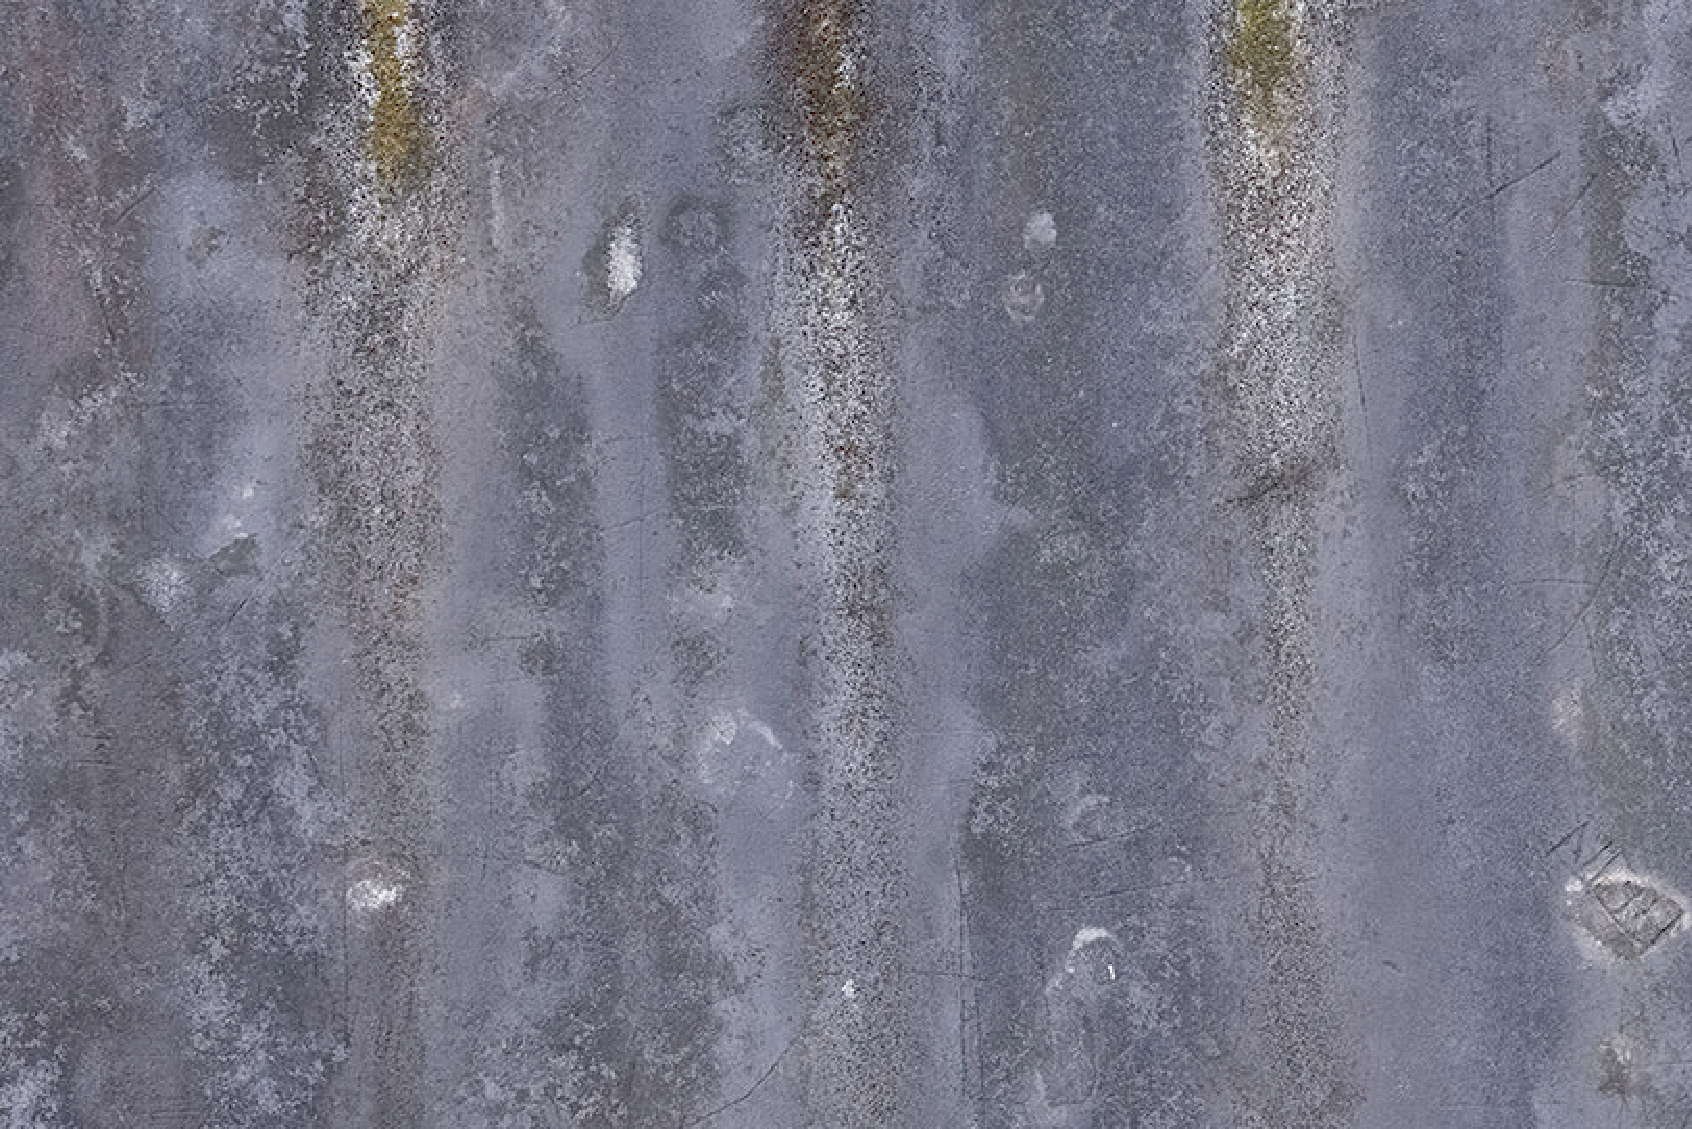
\includegraphics[height=88mm]{ch_back.pdf}};}](O1)-|(O3)-|cycle;
	% イラスト
	%\draw[path picture={\node at (path picture bounding box.center)
		%{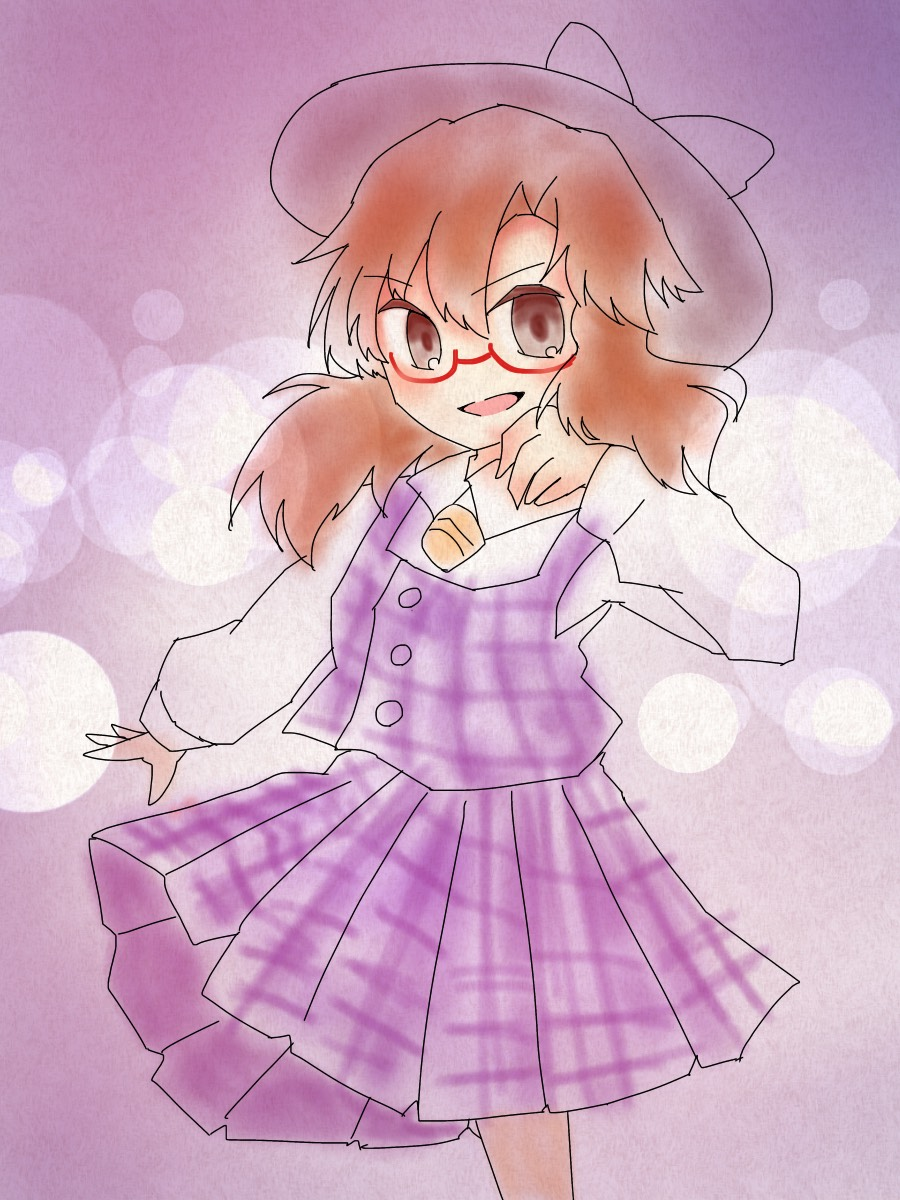
\includegraphics[width=49mm]{sumire.jpg}};}](I1)rectangle(I3);
	\draw[path picture={\node at (path picture bounding box.center)
		{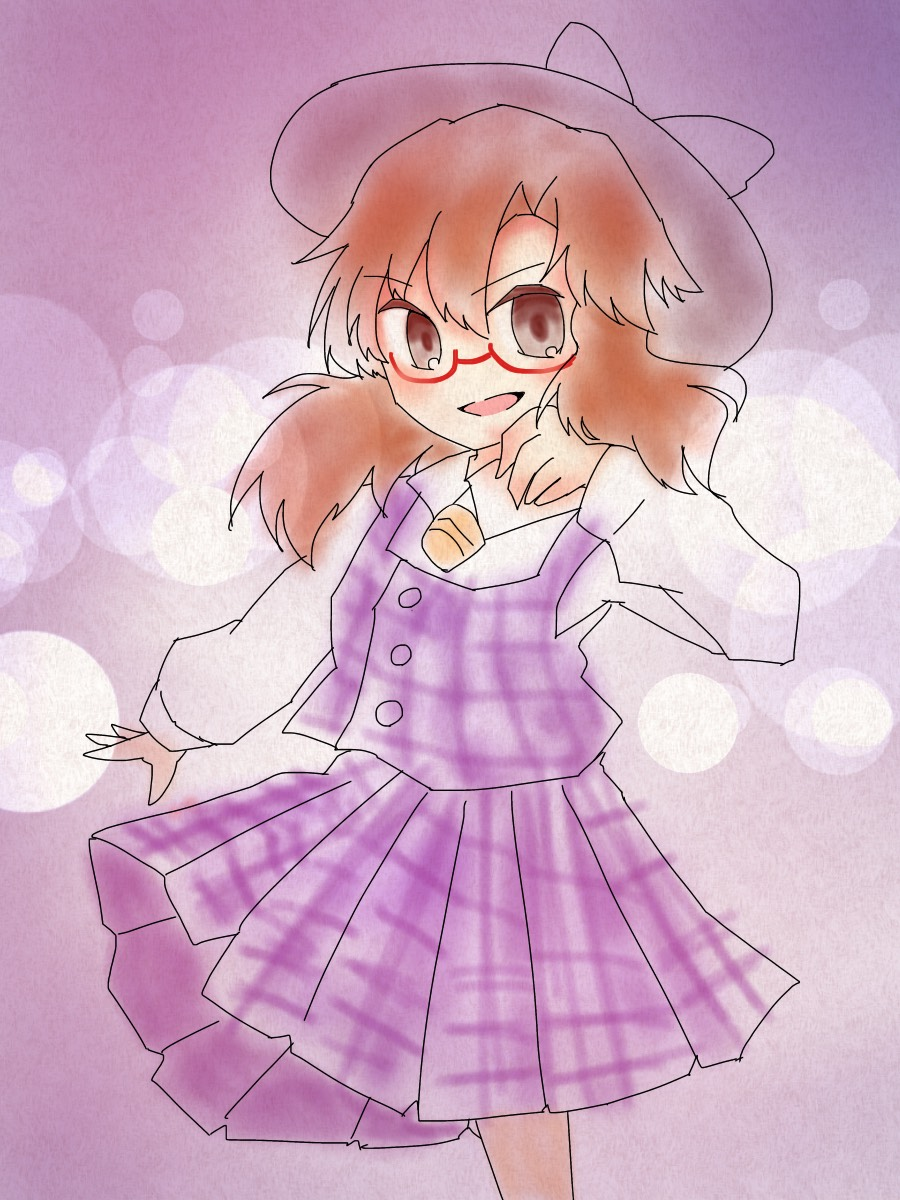
\includegraphics[height=88mm]{sumire.jpg}};}](OL1)rectangle(OL3);
	% カード名
	\fill[black,path fading=west](M1)rectangle(M3);
	\path(MT)node[below,inner sep=0,outer sep=0]
		{\hbox{\tate\hminwidth{48mm}{\fontsize{6mm}{0}\hmnfont\hmfukuro[.3pt]{宇佐見 菫子}}}};
	\path(RT)node[below,white,inner sep=0,outer sep=0]
		{\hbox{\tate\hminwidth*{44mm}{\fontsize{2mm}{0}\hmnfont うさみ すみれこ}}};
	% タイプ、術者
	\filldraw[fill=characolor!50,draw=characolor](TC)circle[radius=1.9];
	\draw(TC)node{\hmtfont{Ch}};
	\path(TC)--++(2,0)node[right]{\hmsfont\hmfukuro{}};
	% コスト
	\filldraw[fill=costcolor!30,draw=costcolor,thick](C1)rectangle(C3);
	\fill[fill=costcolor!70]
		($(C1)!.5!(C2)$)--($(C2)!.5!(C3)$)--($(C3)!.5!(C4)$)--($(C4)!.5!(C1)$)--cycle
		(C1)-|(C3)|-cycle;
	\path(C1)|-(C3)node[near end,above,outer ysep=0]{\hmcfont\small COST};
	\path(C1)--(C3)node[midway]{\hmcfont\Huge\hmfukuro{2}};
	% ノード
	\filldraw[fill=nodecolor!30,draw=nodecolor,thick](N1)rectangle(N3);
	\fill[fill=nodecolor!70](N1)--(N3)--(N4)--(N2)--cycle;
	\path(N1)-|(N3)node[near start,below,outer ysep=0]{\hmcfont\small NODE};
	\path(N1)--(N3)node[midway]{\hmcfont\Huge\hmfukuro{5}};
	% 霊力
	\filldraw[fill=spiritcolor!40,draw=spiritcolor,thick](SC)circle[radius=3];
	\fill[fill=spiritcolor!10](SC)circle[radius=2];
	\path(SC)--++(0,2.5)node{\small\hmgcfont\hmfukuro{\strut Spirit}};
	\path(SC)node{\LARGE\hmgfont 3};
	% グレイズ
	\fill[fill=grazecolor!10](GC)circle[radius=4.5];
	\fill[fill=grazecolor!40](GC)--++(-45:4.5)arc(315:135:4.5)--cycle;
	\draw[draw=grazecolor,thick](GC)circle[radius=4.5];
	\path(GC)--++(0,3.5)node{\small\hmgcfont\hmfukuro{\strut Graze}};
	\path(GC)node{\Huge\hmgfont 3};
	% % 発動期間
	% \filldraw[fill=rangebcolor,draw=rangebcolor!80,thick](SC2)circle[radius=2.5];
	% \path(SC2)node[rangecolor]{\LARGE\hmicot};
	% % 効果範囲
	% \filldraw[fill=rangebcolor,draw=rangebcolor!80,thick](GC2)circle[radius=2.5];
	% \path(GC2)node[rangecolor]{\LARGE\hmicom};
	% 種族
	\path(I3)-|(I1)node[midway,above left]{\large\hmsfont\hmfukuro{人間}};
	% テキスト
	\draw[fill=icoAcolor!30,fill opacity=.85](B1)rectangle(B3);
	%% 場所
	\path(B1)--(B3)node[midway,text opacity=.3]{\fontsize{20mm}{0}\hmicoA};
	%% テキスト
	\path(B1)-|(B3)node[
		midway,below right,outer sep=0,inner sep=1mm,text width=53mm,text justified,font=\small\sffamily]{
			(自動γ)〔このキャラクター〕にセットされているカードが 7 枚以上になった場合、
			〔このキャラクターにセットされているカード全て〕を破棄する。その後、この効果で
			破棄したカードから 1 枚選んで、あなたがプレイしたものとして解決する。
			
			(自分ターン)[2]\↓: 目標の〔あなたの冥界にあるカード 1 枚〕を〔このキャラクター〕
			にセットする。
		};
	%% 戦闘力
	\path($(B1)-(7,0)$)|-(B3)node
		[midway,above,outer sep=0,inner xsep=0,inner ysep=1mm,text width=14mm,text centered,font=\LARGE\hmpfont]
		{\mbox{\makebox[4mm][r]{3}/\makebox[4mm][l]{5}}};
	%% フレーバーテキスト
	\path(B3)node[above right,outer sep=0,inner sep=1mm,text width=39mm,text justified,font=\scriptsize]{
			「捕まえたわー! 夢の中だけど持って帰れるかなぁ」
		};
	% フッター
	\path(O3)node[above right,text width=10\zw,align=left,inner ysep=0,outer ysep=0]
		{\hmfukuro{\scriptsize\hmsfont{\©}上海アリス幻樂団\\[-3pt]{\©}さーくる⑨}};
	\path(O1)|-(O3)node[pos=.75,above left,inner xsep=0,outer xsep=0]{\hmpfont\small\hmfukuro{PR.~}};
	\path(O1)|-(O3)node[pos=.75,above right,inner xsep=0,outer xsep=0]{\hmpfont\small\hmfukuro{0001}};
	\path(O1)|-(O3)node[pos=.68,above]{\hmpfont\small\hmfukuro{<S>}};
	\path(O1)|-(O3)node[midway,above left]{\hmsfont\small\hmfukuro{Ill. 湯島}};
	% % 方眼
	% \draw[very thin,gridcolor,nearly transparent](OL1)grid[step=1](OL3);
	% \draw[gridcolor,nearly transparent]($(OL1)-(2,2)$)rectangle($(OL3)+(2,2)$);
	% \draw[thin,gridcolor,nearly transparent](OL1)grid[step=10](OL3);
	% \draw[thin,gridcolor,nearly transparent](OL1)rectangle(OL3);
\end{tikzpicture}
\end{document}
